Let $N$ be the number of vertices in the free tree.

To solve this problem, we will use an algorithm in two steps: in the first step we will gather and store the information needed in the second step to compute the balance of each vertex.

To compute the balance of a vertex $V_i$, all what we need to compute in the first step is the number of vertices in the isolated trees connected to the vertex $V_i$. For every vertex $V_j$ connected to the vertex $V_i$, we want to compute $N_{i,j}$ the number of vertices in the isolated tree containing the vertex $V_j$ from the point of view of $V_i$.

If we know that the vertex $V_i$ is connected to the vertex $V_j$, if from the point of view of $V_i$ there are $N_{i,j}$ vertices in the isolated tree containing $V_j$, then from the point of view of $V_j$, there are $N_{j,i} = N - N_{i,j}$ vertices in the isolated tree containing $V_i$.
For each pair $(i,j)$ we only need to know $N_{i,j}$ or $N_{j,i}$ to know the other one.

That is why our first step is just a depth first search (starting from any vertex), during which we compute recursively and store the $N_{i,j}$ (and $N_{j,i}$ by complementing to $N$) for every connected vertices, like on the figure 1:

\begin{figure}[h!]
\begin{center}
   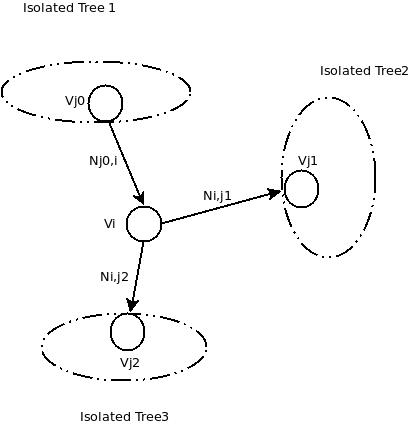
\includegraphics[width=8cm]{IsolatedTreesDFS}
   \caption{We come from the vertex $V_{j0}$ of the isolated tree 1, go to vertex $V_i$. $N_{j0,i} = N_{i,j1} + N_{i,j2} + 1$}
\end{center}
\end{figure}

This step runs in $\Theta(N)$.

After this step, we just need to find the vertex with the lowest balance by doing another search on the free tree, as we can know compute the balance of a vertex $V_i$ as the maximum of the $N_{i,j}$ we have computed before.

This step also runs in $\Theta(N)$, and our algorithm is linear.